\documentclass[aspectratio=169, 10pt]{beamer}

% --- Tipografía y Lenguaje ---
\usepackage{fontspec}
\usepackage[spanish, es-tabla]{babel}

% --- Paquetes Matemáticos y Gráficos ---
\usepackage{amsmath, amsfonts, amssymb}
\usepackage{booktabs}
\usepackage{colortbl}
\usepackage{graphicx}
\usepackage{microtype}
\usepackage{tcolorbox}
\usepackage{tikz}
\usetikzlibrary{positioning}
\tcbuselibrary{skins, hooks}

% --- Configuración de Rutas de Figuras ---
\graphicspath{{../memoria/figures/}{./figures/}}

% --- Colores Corporativos UPV y Sistema ---
\definecolor{UPVNavy}{RGB}{0, 40, 85}
\definecolor{UPVRed}{RGB}{192, 0, 0}
\definecolor{DarkSlate}{RGB}{30, 41, 59}
\definecolor{LightSlate}{RGB}{248, 250, 252}
\definecolor{BorderGray}{RGB}{226, 232, 240}
\definecolor{EmeraldGreen}{RGB}{16, 185, 129}
\definecolor{CobaltBlue}{RGB}{37, 99, 235}
\definecolor{AmberWarning}{RGB}{245, 158, 11}
\definecolor{CrimsonError}{RGB}{239, 68, 68}

% --- Configuración del Tema Metropolis ---
\usetheme[progressbar=frametitle, block=fill]{metropolis}

% Personalización de la paleta
\setbeamercolor{normal text}{fg=DarkSlate, bg=white}
\setbeamercolor{palette primary}{bg=UPVNavy, fg=white}
\setbeamercolor{progress bar}{fg=UPVRed, bg=UPVNavy!20}
\setbeamercolor{title separator}{fg=UPVRed}
\setbeamercolor{frametitle}{bg=white, fg=UPVNavy}
\setbeamercolor{alerted text}{fg=UPVRed}
\setbeamercolor{example text}{fg=EmeraldGreen}

\setbeamertemplate{navigation symbols}{}
\setbeamercovered{transparent}

% --- Componentes UI Modernos (Cards, Badges, StatBoxes) ---
\newtcolorbox{statbox}[3][]{
  enhanced,
  colback=white,
  colframe=#3,
  coltitle=white,
  arc=3mm,
  boxrule=1pt,
  leftrule=4pt,
  width=\linewidth,
  boxsep=2pt,
  top=4pt,
  bottom=4pt,
  left=6pt,
  right=6pt,
  shadow={0.5mm}{-0.5mm}{0mm}{black!8},
  title={\small\textbf{#2}},
  #1
}

\newtcolorbox{metriccard}[2][]{
  enhanced,
  colback=#2!6,
  colframe=#2,
  boxrule=0.8pt,
  leftrule=3.5pt,
  arc=2mm,
  boxsep=2pt,
  top=4pt,
  bottom=4pt,
  left=6pt,
  right=6pt,
  #1
}

\newtcolorbox{herocard}[1][]{
  enhanced,
  colback=UPVNavy!5,
  colframe=UPVNavy,
  boxrule=0.8pt,
  leftrule=4pt,
  arc=2.5mm,
  boxsep=3pt,
  top=5pt,
  bottom=5pt,
  left=8pt,
  right=8pt,
  #1
}

\newcommand{\badge}[2]{%
  \tcbox[on line, boxrule=0pt, boxsep=1pt, top=1pt, bottom=1pt, left=4pt, right=4pt, colback=#2!15, colframe=#2!15, arc=2mm]{%
    \scriptsize\textcolor{#2}{\textbf{#1}}%
  }%
}

\newcommand{\cmark}{\textcolor{EmeraldGreen}{\textbf{\checkmark}}}
\newcommand{\xmark}{\textcolor{CrimsonError}{\textbf{$\times$}}}

% --- Metadatos de la Presentación ---
\title{\textbf{Sistema de Predicción de Demanda para Retail con Análisis de Incertidumbre}}
\subtitle{Modelado de Demanda Censurada, Calibración Conformal y Optimización Newsvendor}
\author{\textbf{Artem Mindlin}}
\institute{
  \textbf{Grado en Ciencia de Datos}\\
  Escuela Técnica Superior de Ingeniería Informática (ETSINF)\\
  Universitat Politècnica de València (UPV)
}
\date{Valencia, Septiembre de 2026}

\begin{document}

% ==============================================================================
% PORTADA
% ==============================================================================
\begin{frame}[plain]
  \titlepage
\end{frame}

% ==============================================================================
% AGENDA / ÍNDICE
% ==============================================================================
\begin{frame}{Estructura de la Defensa}
  \begin{columns}[T]
    \begin{column}{0.48\textwidth}
      \begin{metriccard}{UPVNavy}
        \textbf{\textcolor{UPVNavy}{01. Contexto y Desafío}}
        \begin{itemize}\small
          \item Asimetría de costes en perecederos
          \item Censura de demanda y fallo del MAE
          \item Objetivos y KPIs de validación
        \end{itemize}
      \end{metriccard}
      \vspace{0.2cm}
      \begin{metriccard}{CobaltBlue}
        \textbf{\textcolor{CobaltBlue}{02. Metodología y Formulación}}
        \begin{itemize}\small
          \item Pipeline modular end-to-end
          \item Imputación supervisada de censura
          \item Mondrian Conformal Prediction
          \item Decisión de inventario Newsvendor
        \end{itemize}
      \end{metriccard}
    \end{column}
    \begin{column}{0.48\textwidth}
      \begin{metriccard}{EmeraldGreen}
        \textbf{\textcolor{EmeraldGreen}{03. Resultados Experimentales}}
        \begin{itemize}\small
          \item La trampa del MAE frente al coste
          \item Optimización biobjetivo (Pareto)
          \item Validación económica y streaming
          \item Explicabilidad global (SHAP)
        \end{itemize}
      \end{metriccard}
      \vspace{0.2cm}
      \begin{metriccard}{UPVRed}
        \textbf{\textcolor{UPVRed}{04. Plataforma MLOps y Cierre}}
        \begin{itemize}\small
          \item Arquitectura web DSS (Django/HTMX)
          \item Limitaciones y líneas futuras
          \item Impacto en sostenibilidad (ODS 12/13)
        \end{itemize}
      \end{metriccard}
    \end{column}
  \end{columns}
\end{frame}

% ==============================================================================
% SECCIÓN 1
% ==============================================================================
\begin{frame}[standout]
  \Huge \textbf{01} \\[0.4cm]
  \Large \textbf{Contexto y Desafío del Retail} \\[0.2cm]
  \normalsize El problema de reposición en productos frescos
\end{frame}

\begin{frame}{El Problema Logístico: Asimetría y Desperdicio}
  \begin{columns}[T]
    \begin{column}{0.48\textwidth}
      \begin{statbox}{El Negocio de Perecederos}{UPVNavy}
        \begin{itemize}\small
          \item \textbf{Alta Volatilidad:} Vida útil corta (días) y demanda altamente sensible a estacionalidad.
          \item \textbf{Costes Asimétricos:}
          \begin{itemize}\footnotesize
            \item Coste por rotura (\textit{understock} $c_u$): Pérdida de margen y fuga de clientes.
            \item Coste por exceso (\textit{overstock} $c_o$): Merma total y coste de gestión de residuo.
          \end{itemize}
          \item \textbf{Impacto Regulatorio:} Ley 1/2025 de prevención de pérdidas y desperdicio alimentario.
        \end{itemize}
      \end{statbox}
    \end{column}
    \begin{column}{0.48\textwidth}
      \begin{statbox}{Los Dos Cuellos de Botella Técnicos}{UPVRed}
        \begin{itemize}\small
          \item \textbf{1. Censura de Demanda por Rotura:}\\
          Cuando hay stockout ($I_t = 0$), las ventas caen a cero. El dato observado \textbf{no refleja el deseo real de compra}.
          \item \textbf{2. La Trampa del Error Medio:}\\
          Minimizar MAE/RMSE persigue la media o mediana condicional, ignorando la asimetría financiera $c_u \gg c_o$.
        \end{itemize}
      \end{statbox}
    \end{column}
  \end{columns}
\end{frame}

\begin{frame}{Objetivos Específicos y Validación de KPIs}
  \begin{table}[h]
    \centering
    \small
    \begin{tabular}{lllcc}
      \toprule
      \textbf{KPI} & \textbf{Métrica / Descripción} & \textbf{Objetivo} & \textbf{Resultado} & \textbf{Estado} \\
      \midrule
      \textbf{KPI-1} & Cobertura empírica conformal & $\ge 80{,}0\%$ a $\alpha=0{,}2$ & \textbf{85,5\%} & \cmark \\
      \textbf{KPI-2} & Reducción de coste Newsvendor & Ahorro $> 0\%$ vs Naïve & \textbf{-9,03\%} & \cmark \\
      \textbf{KPI-3} & Imputación demanda latente & Reconstrucción sin data leak & \textbf{-92,15\%} coste & \cmark \\
      \textbf{KPI-4} & Retención de servicio en drift & Fill rate en streaming & \textbf{95,43\%} & \cmark \\
      \textbf{KPI-5} & Calidad de ingeniería de software & Tests automatizados & \textbf{309 / 309} & \cmark \\
      \textbf{KPI-6} & Latencia de reentreno operacional & $< 10$ s / ciclo streaming & \textbf{5,55 s} & \cmark \\
      \bottomrule
    \end{tabular}
  \end{table}
  \vspace{0.2cm}
  \begin{herocard}
    \small \textbf{Benchmark de Evaluación:} \textit{FreshRetailNet-50K} (Mayo 2025) · 50.000 series temporales a nivel SKU-tienda, evaluado sobre el subset de \textbf{500 series de alta rotación}.
  \end{herocard}
\end{frame}

% ==============================================================================
% SECCIÓN 2
% ==============================================================================
\begin{frame}[standout]
  \Huge \textbf{02} \\[0.4cm]
  \Large \textbf{Metodología y Formulación Matemática} \\[0.2cm]
  \normalsize Uniendo Machine Learning, Inferencia Conformal e Investigación Operativa
\end{frame}

\begin{frame}{Arquitectura Metodológica Modular}
  \centering
  \begin{tikzpicture}[node distance=0.8cm, auto, >=stealth, font=\footnotesize]
    \tikzstyle{block} = [rectangle, draw=UPVNavy, fill=UPVNavy!8, text width=2.1cm, text centered, rounded corners=2mm, minimum height=1.2cm, line width=0.8pt]
    \tikzstyle{arrow} = [thick, ->, >=stealth, color=UPVNavy]

    \node [block] (data) {\textbf{1. Datos Brutos}\\\scriptsize FreshRetailNet-50K\\(Ventas censuradas)};
    \node [block, right=0.25cm of data] (impute) {\textbf{2. Imputador}\\\scriptsize LightGBM supervisado\\$\hat{D}_t$ latente};
    \node [block, right=0.25cm of impute] (ml) {\textbf{3. Forecasting}\\\scriptsize GBDT Cuantílico\\$\hat{y}_{t+h}$ puntual};
    \node [block, right=0.25cm of ml] (conformal) {\textbf{4. Conformal}\\\scriptsize Mondrian CP\\Intervalos $[q_{0.1}, q_{0.9}]$};
    \node [block, right=0.25cm of conformal] (decision) {\textbf{5. Newsvendor}\\\scriptsize Pedido óptimo $q^*$\\Coste logístico};

    \draw [arrow] (data) -- (impute);
    \draw [arrow] (impute) -- (ml);
    \draw [arrow] (ml) -- (conformal);
    \draw [arrow] (conformal) -- (decision);
  \end{tikzpicture}

  \vspace{0.4cm}
  \begin{columns}[T]
    \begin{column}{0.48\textwidth}
      \begin{metriccard}{CobaltBlue}
        \textbf{\textcolor{CobaltBlue}{Principios de Diseño Causal}}
        \begin{itemize}\footnotesize
          \item \textbf{Zero-Leakage Guarantee:} Ninguna información censurada por stockout contamina la etiqueta objetivo futura.
          \item \textbf{Embargo Temporal:} Ventana de guarda para evitar solapamientos entre calibración e inferencia.
        \end{itemize}
      \end{metriccard}
    \end{column}
    \begin{column}{0.48\textwidth}
      \begin{metriccard}{EmeraldGreen}
        \textbf{\textcolor{EmeraldGreen}{Optimización Integral de Decisión}}
        \begin{itemize}\footnotesize
          \item No se optimiza para error cuadrático medio.
          \item Toda la sintonización (\textit{tuning}) persigue minimizar directamente el \textbf{coste monetario de inventario}.
        \end{itemize}
      \end{metriccard}
    \end{column}
  \end{columns}
\end{frame}

\begin{frame}{Imputación Supervisada de Demanda Latente}
  \begin{columns}[c]
    \begin{column}{0.50\textwidth}
      \begin{statbox}{Formulación del Problema}{UPVNavy}
        Demanda observada $Y_t$ condicionada al stock $I_t$:
        $$Y_t = \begin{cases} D_t & \text{si } I_t > 0 \text{ (sin rotura)} \\ \min(D_t, I_t) & \text{si } I_t = 0 \text{ (censurada)} \end{cases}$$
      \end{statbox}
      \begin{statbox}{Estrategia de Modelado}{EmeraldGreen}
        \begin{itemize}\small
          \item \textbf{Fase de Entrenamiento:} Entrenar un regresor $G(X_t)$ exclusivamente sobre periodos limpios ($I_t > 0$).
          \item \textbf{Fase de Inferencia:} Estimar $\hat{D}_t = G(X_t)$ en periodos con stockout.
          \item Preserva señales estacionales, calendario y rezagos limpios.
        \end{itemize}
      \end{statbox}
    \end{column}
    \begin{column}{0.46\textwidth}
      \begin{herocard}
        \textbf{\textcolor{UPVNavy}{Aportación Metodológica}}
        \vspace{0.2cm}
        \begin{itemize}\small
          \item Demostración de que el protocolo de censura sintética es \textbf{circular} si solo se evalúa sobre días truncados artificialmente.
          \item Necesidad imperativa de una \textbf{evaluación bajo verdad común} sobre el coste de inventario.
        \end{itemize}
      \end{herocard}
    \end{column}
  \end{columns}
\end{frame}

\begin{frame}{Calibración con Mondrian Conformal Prediction}
  \begin{columns}[T]
    \begin{column}{0.50\textwidth}
      \begin{statbox}{Garantía Conformal en Muestra Finita}{UPVNavy}
        Para un nivel de significancia $\alpha = 0{,}20$ (cobertura nominal del $80\%$):
        $$P(Y_{n+1} \in \hat{C}(X_{n+1})) \ge 1 - \alpha$$
        \begin{itemize}\footnotesize
          \item \textbf{Score de No-Conformidad:} Residuos estandarizados por la incertidumbre estimada.
          \item \textbf{Estratificación Mondrian:} Calibración independiente por conglomerados de rotación/volatilidad para evitar sesgos entre categorías.
        \end{itemize}
      \end{statbox}
    \end{column}
    \begin{column}{0.46\textwidth}
      \begin{statbox}{Decisión Newsvendor Asimétrica}{EmeraldGreen}
        Fractil crítico derivado del equilibrio financiero:
        $$\tau = \frac{c_u}{c_u + c_o} = \frac{4{,}0}{4{,}0 + 1{,}0} = 0{,}80$$
        $$q^* = \hat{F}_D^{-1}(\tau) = \hat{y}_{\text{pred}} + \hat{s}_{\text{conformal}}(\tau)$$
        \begin{itemize}\footnotesize
          \item El cuantil conformal $\hat{s}(\tau)$ absorbe la asimetría económica de las pérdidas.
        \end{itemize}
      \end{statbox}
    \end{column}
  \end{columns}
\end{frame}

% ==============================================================================
% SECCIÓN 3
% ==============================================================================
\begin{frame}[standout]
  \Huge \textbf{03} \\[0.4cm]
  \Large \textbf{Resultados Experimentales y Evaluación} \\[0.2cm]
  \normalsize Evidencia empírica sobre 500 series en backtesting walk-forward
\end{frame}

\begin{frame}{La Trampa del MAE: Error Predictivo vs Impacto Real}
  \begin{columns}[c]
    \begin{column}{0.45\textwidth}
      \centering
      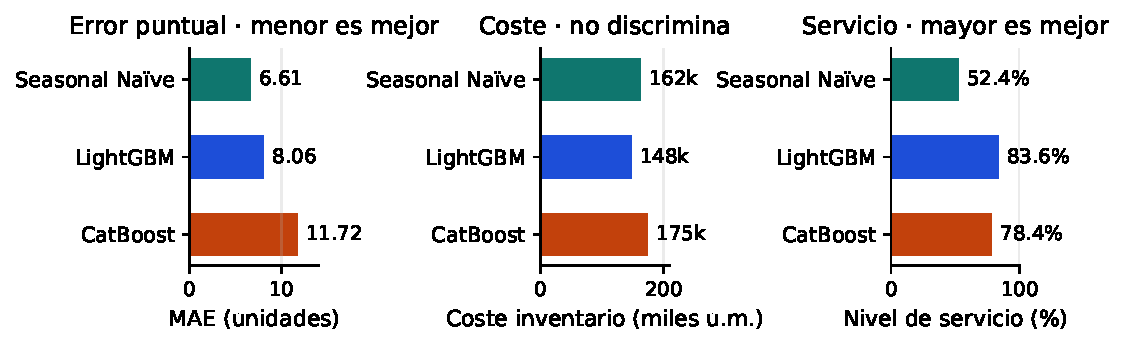
\includegraphics[width=\linewidth,height=0.72\textheight,keepaspectratio]{mae_vs_servicio.pdf}
    \end{column}
    \begin{column}{0.52\textwidth}
      \begin{statbox}{El Hallazgo Crítico}{UPVRed}
        \begin{itemize}\small
          \item \textbf{Seasonal Naïve} obtiene el mejor MAE ($6{,}61$) porque predice la mediana condicional.
          \item Sin embargo, genera rotura masiva: \textbf{$52{,}45\%$ de nivel de servicio} (falla en casi la mitad de los días).
          \item \textbf{LightGBM Conformal} eleva el nivel de servicio a \textbf{$83{,}55\%$} ($+31{,}10$ p.p.) con el menor coste logístico ($147.646$ u.m.).
        \end{itemize}
      \end{statbox}
    \end{column}
  \end{columns}
\end{frame}

\begin{frame}{Tabla Comparativa: Backtesting Walk-Forward ($K=3, H=7$)}
  \begin{table}[h]
    \centering
    \footnotesize
    \begin{tabular}{lcccccc}
      \toprule
      \textbf{Modelo} & \textbf{MAE} & \textbf{RMSE} & \textbf{Winkler (80\%)} & \textbf{Coste (u.m.)} & \textbf{Nivel Servicio} & \textbf{Cobertura} \\
      \midrule
      \textbf{Seasonal Naïve} & \textbf{6,61} & \textbf{8,90} & n/a & 162.299 & 52,45\% & n/a \\
      \textbf{CatBoost} & 11,72 & 16,87 & 46,54 & 174.527 & 78,39\% & 84,6\% \\
      \textbf{LightGBM (Campeón)} & 8,06 & 10,82 & \textbf{36,11} & \textbf{147.646} & \textbf{83,55\%} & \textbf{85,5\%} \\
      \bottomrule
    \end{tabular}
  \end{table}

  \begin{columns}[T]
    \begin{column}{0.32\textwidth}
      \begin{metriccard}{CobaltBlue}
        \centering
        \textbf{\large -9,03\%}\\[0.1cm]
        \scriptsize Reducción de coste vs Naïve\\(IC95: $[-15{,}5\%, -2{,}7\%]$)
      \end{metriccard}
    \end{column}
    \begin{column}{0.32\textwidth}
      \begin{metriccard}{EmeraldGreen}
        \centering
        \textbf{\large +31,10 p.p.}\\[0.1cm]
        \scriptsize Incremento en nivel de servicio\\(52,45\% $\rightarrow$ 83,55\%)
      \end{metriccard}
    \end{column}
    \begin{column}{0.32\textwidth}
      \begin{metriccard}{UPVNavy}
        \centering
        \textbf{\large 36,11}\\[0.1cm]
        \scriptsize Winkler Score más compacto\\(19\% más estrecho que CatBoost)
      \end{metriccard}
    \end{column}
  \end{columns}
\end{frame}

\begin{frame}{Optimización Biobjetivo y Estabilidad Fuera de Muestra}
  \begin{columns}[c]
    \begin{column}{0.55\textwidth}
      \centering
      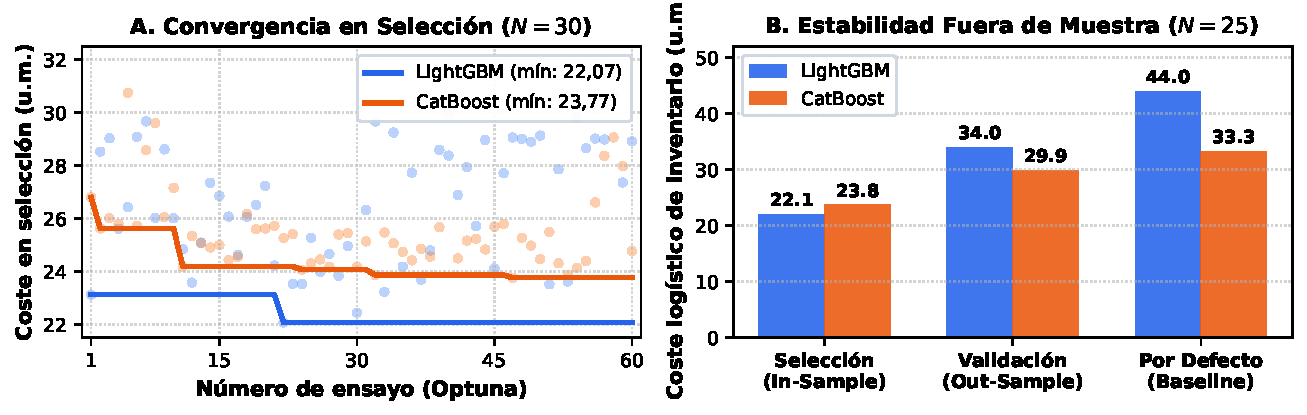
\includegraphics[width=\linewidth,height=0.72\textheight,keepaspectratio]{tuning_comparison_60trials.pdf}
    \end{column}
    \begin{column}{0.42\textwidth}
      \begin{statbox}{Protocolo Desacoplado}{UPVNavy}
        \begin{itemize}\small
          \item \textbf{60 Ensayos MOTPE (Optuna):} Búsqueda en frente de Pareto (Coste vs Winkler).
          \item \textbf{Validación Fuera de Muestra ($N=25$ sorteos):}
          \begin{itemize}\footnotesize
            \item LightGBM gana \textbf{-22,66\%} en validación frente a parámetros default.
            \item CatBoost gana \textbf{-10,01\%}.
          \end{itemize}
          \item Evita sobreajuste a la ventana de selección.
        \end{itemize}
      \end{statbox}
    \end{column}
  \end{columns}
\end{frame}

\begin{frame}{Evaluación Financiera de Demanda Latente}
  \begin{statbox}{Comparativa Bajo Verdad Común no Censurada ($N=500$ series)}{EmeraldGreen}
    \centering\small
    Evaluación del coste monetario según el tratamiento de la señal censurada.
  \end{statbox}
  \vspace{0.1cm}
  \begin{table}[h]
    \centering
    \footnotesize
    \begin{tabular}{lcccc}
      \toprule
      \textbf{Estrategia de Datos} & \textbf{Coste Total (u.m.)} & \textbf{Rotura (uds)} & \textbf{Sobrestock (uds)} & \textbf{Ahorro (\%)} \\
      \midrule
      \textbf{Observed (Ventas crudas)} & 48.910 & 11.240 & 950 & Base (0\%) \\
      \textbf{Zero-filled} & 52.340 & 12.450 & 540 & +7,01\% (peor) \\
      \textbf{Heuristic Imputed} & 18.200 & 3.810 & 2.960 & -62,79\% \\
      \textbf{Latent Supervised (LGBM)} & \textbf{3.839} & \textbf{540} & \textbf{1.679} & \textbf{-92,15\%} \\
      \bottomrule
    \end{tabular}
  \end{table}

  \begin{herocard}
    \small \textbf{Conclusión de Negocio:} Entrenar sobre demanda latente imputada reduce el coste logístico un \textbf{-92,15\%} frente al sesgo de ventas observadas.
  \end{herocard}
\end{frame}

\begin{frame}{Explicabilidad Global del Campeón (SHAP Beeswarm)}
  \begin{columns}[c]
    \begin{column}{0.50\textwidth}
      \centering
      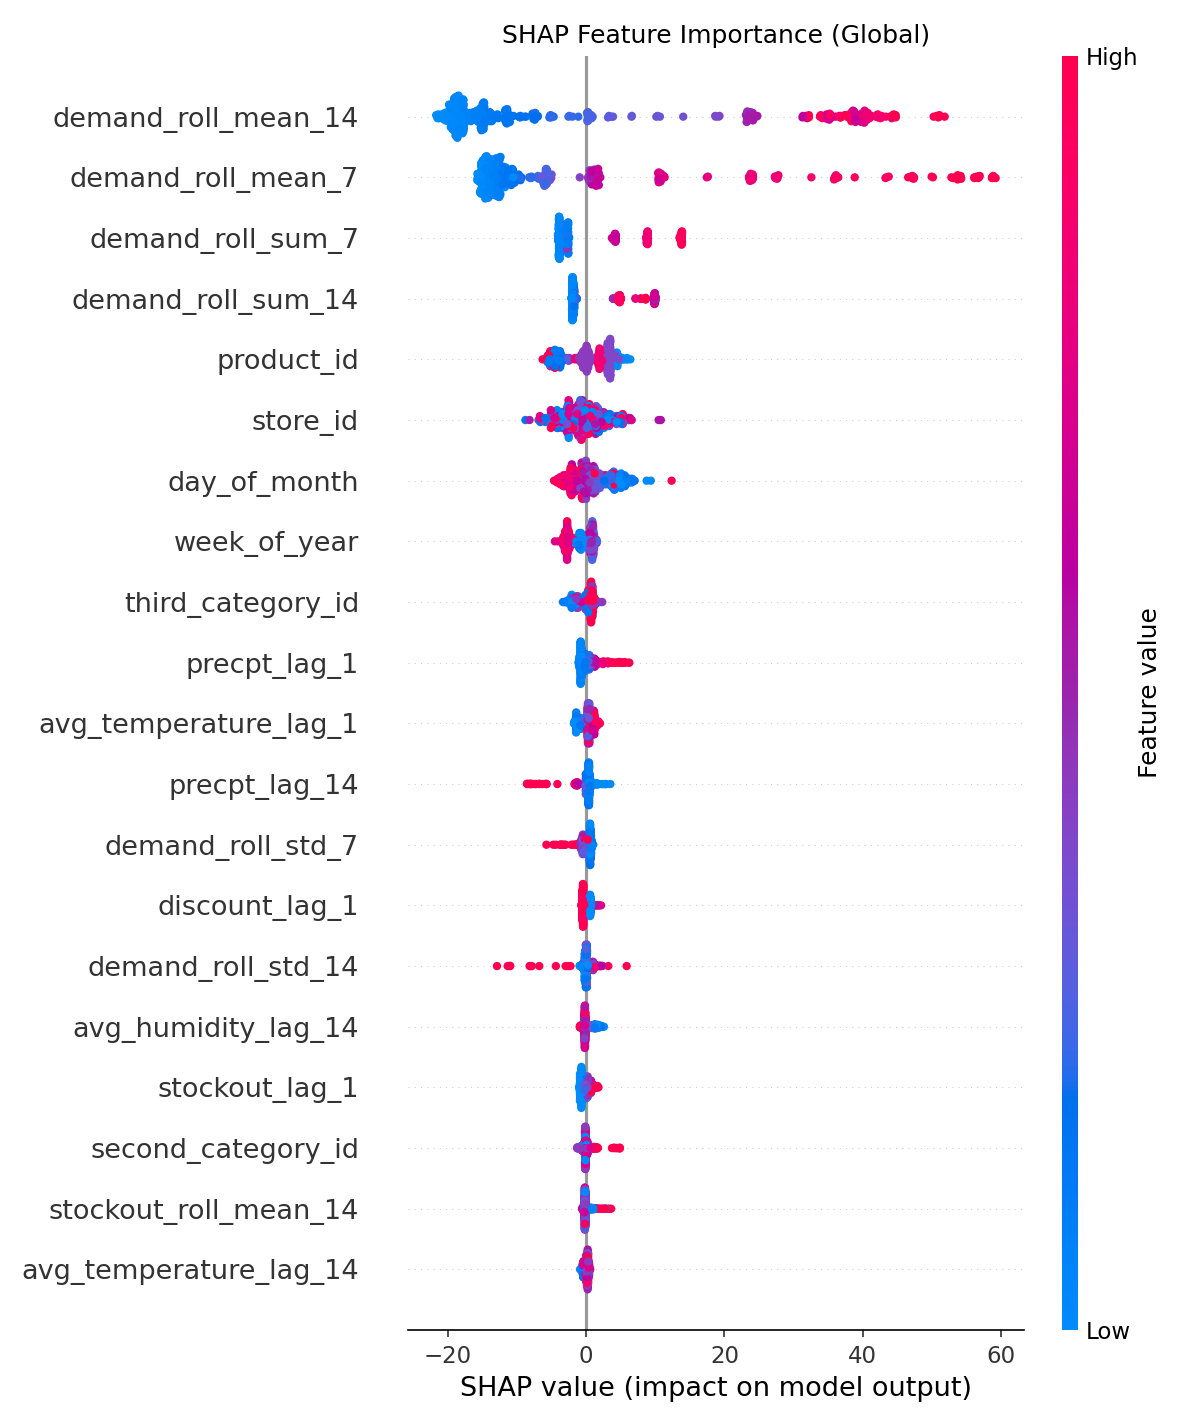
\includegraphics[width=\linewidth,height=0.72\textheight,keepaspectratio]{shap_summary.png}
    \end{column}
    \begin{column}{0.46\textwidth}
      \begin{statbox}{Interpretación del Modelo}{UPVNavy}
        \begin{itemize}\small
          \item \textbf{Features Dominantes:} Las medias móviles de demanda corta ($7$ y $14$ días) dominan el impacto predictivo.
          \item \textbf{Señales Estáticas:} Identificadores de tienda y categoría aportan la base de escala.
          \item \textbf{Transparencia Regulatoria:} Cumplimiento del principio de explicabilidad exigido por el \textit{EU AI Act}.
        \end{itemize}
      \end{statbox}
    \end{column}
  \end{columns}
\end{frame}

\begin{frame}{Simulación Operacional en Streaming y Drift}
  \begin{columns}[c]
    \begin{column}{0.48\textwidth}
      \centering
      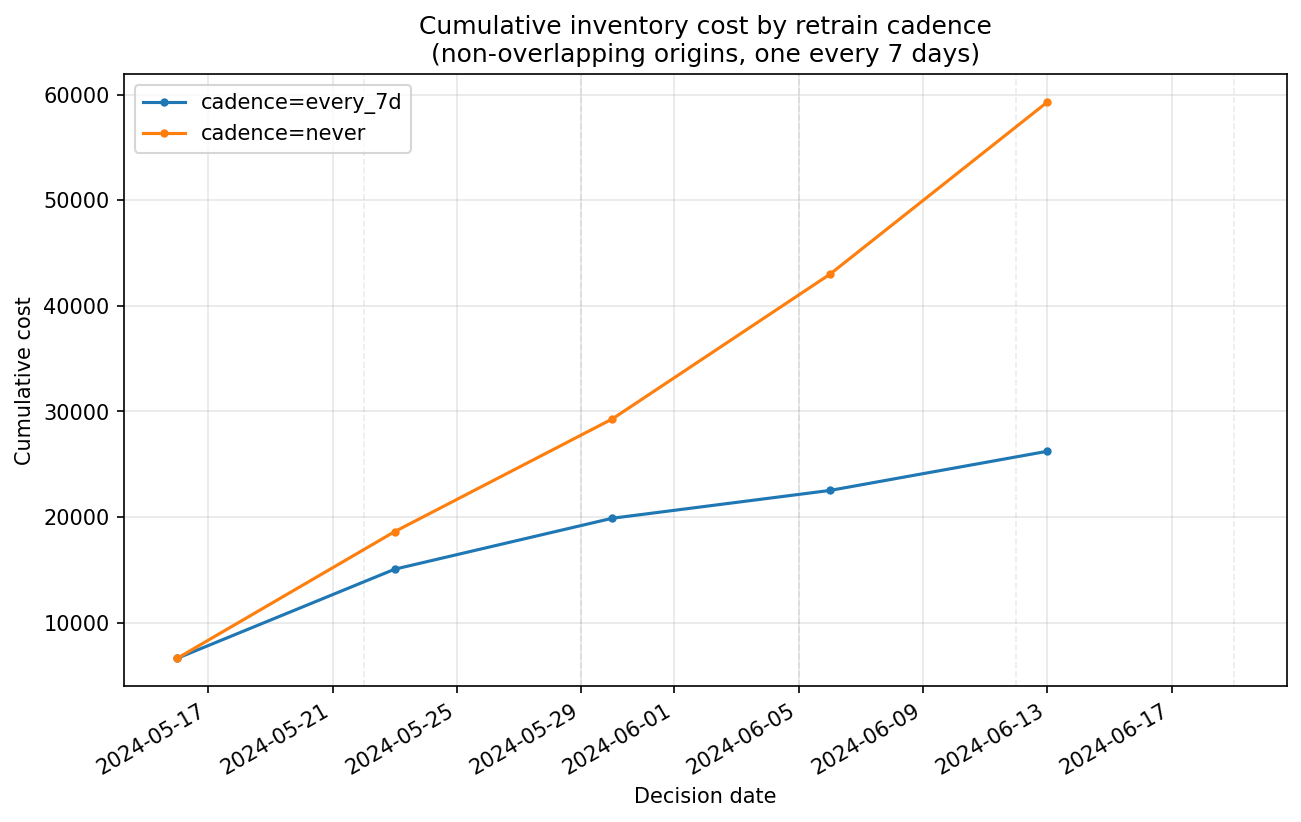
\includegraphics[width=\linewidth,height=0.72\textheight,keepaspectratio]{cumulative_cost.png}
    \end{column}
    \begin{column}{0.48\textwidth}
      \begin{statbox}{Simulación Prequencial (41 días no vistos)}{UPVNavy}
        \begin{itemize}\small
          \item \textbf{Política `never` (estático):}
          Coste $105.676{,}74$ u.m. | Fill Rate $89{,}64\%$
          \item \textbf{Política `every\_7d` (reentreno semanal):}
          Coste \textbf{63.112,52 u.m.} | Fill Rate \textbf{95,43\%}
          \item \textbf{Ahorro Operativo:} \textbf{-40,28\%} ($\Delta = -42.564$ u.m.)
          \item \textbf{Latencia de Reentreno:} Apenas \textbf{5,55 segundos}.
        \end{itemize}
      \end{statbox}
    \end{column}
  \end{columns}
\end{frame}

% ==============================================================================
% SECCIÓN 4
% ==============================================================================
\begin{frame}[standout]
  \Huge \textbf{04} \\[0.4cm]
  \Large \textbf{Plataforma Web y Ciclo de Vida MLOps} \\[0.2cm]
  \normalsize De los experimentos estadísticos a la herramienta de soporte a la decisión
\end{frame}

\begin{frame}{Plataforma Web Operacional (Django + HTMX + Alpine.js)}
  \begin{columns}[c]
    \begin{column}{0.45\textwidth}
      \begin{statbox}{Decision Support System (DSS)}{UPVNavy}
        \begin{itemize}\small
          \item \textbf{Simulador What-If Reactivo:}
          Recálculo instantáneo de pedidos $q^*$ variando parámetros de coste ($c_u, c_o$) en cliente sin recarga.
          \item \textbf{Almacén de Corridas MLflow:}
          Versionado de modelos, métricas y hashes de configuración.
          \item \textbf{API REST Operativa:}
          Endpoints de inferencia JSON por lotes y descarga de reportes.
        \end{itemize}
      \end{statbox}
    \end{column}
    \begin{column}{0.52\textwidth}
      \centering
      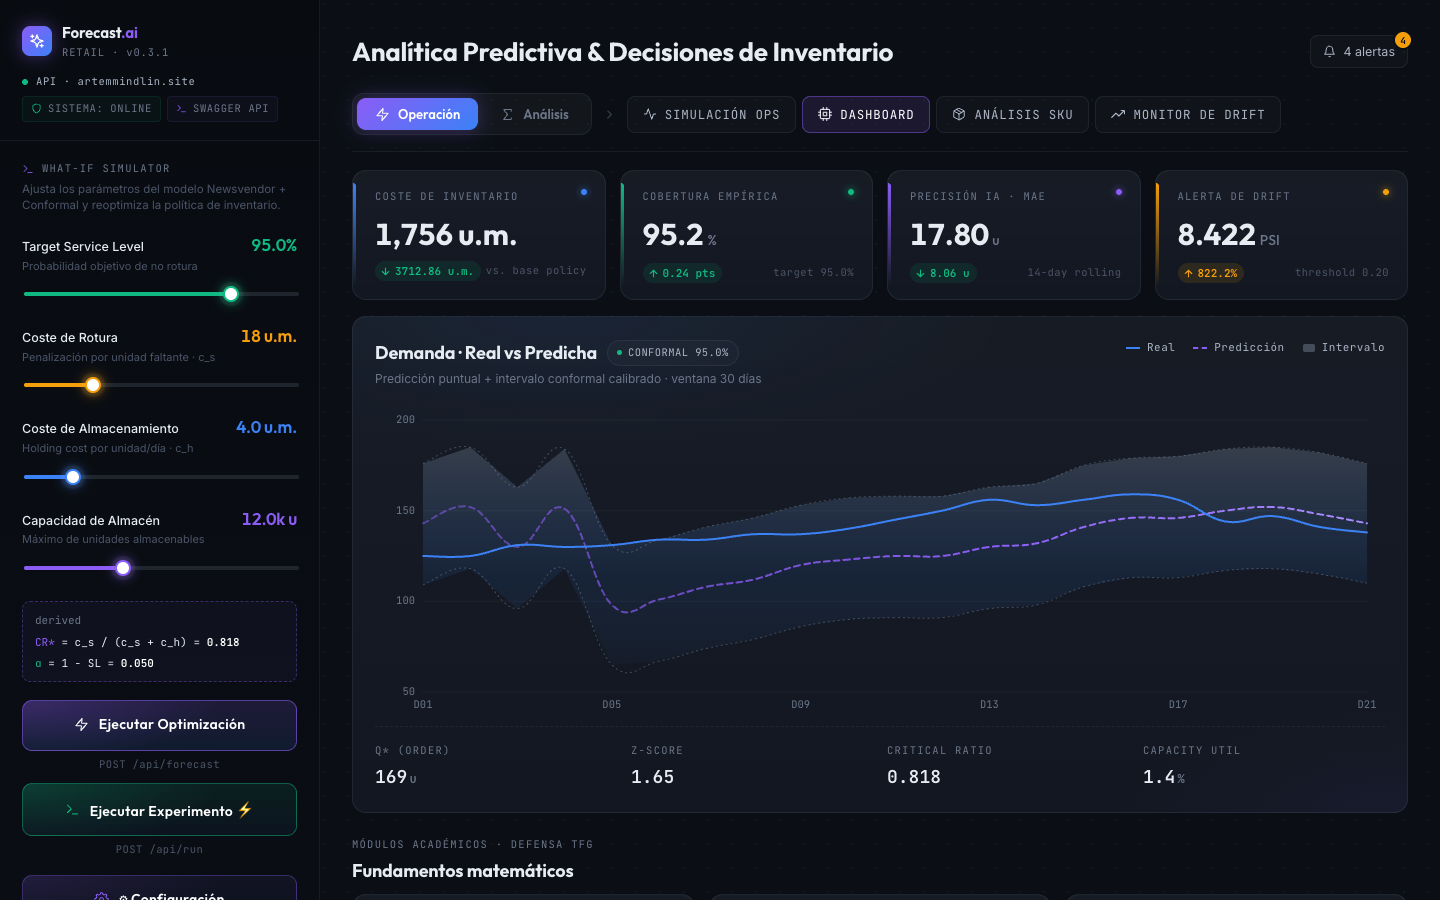
\includegraphics[width=\linewidth,height=0.72\textheight,keepaspectratio]{dashboard/ui_operacion_dashboard.png}
    \end{column}
  \end{columns}
\end{frame}

\begin{frame}{Garantías de Calidad de Software y CI/CD}
  \begin{columns}[T]
    \begin{column}{0.48\textwidth}
      \begin{metriccard}{UPVNavy}
        \textbf{\textcolor{UPVNavy}{Suite de Tests y Contratos}}
        \begin{itemize}\small
          \item \textbf{309 tests automáticos} en pytest (cobertura $>80\%$).
          \item \textbf{Data Quality Gateways:} Validación estricta de esquemas y tipos en cada etapa del pipeline.
          \item \textbf{Temporal Invariant Tests:} Blindaje matemático contra fugas de información.
        \end{itemize}
      \end{metriccard}
    \end{column}
    \begin{column}{0.48\textwidth}
      \begin{metriccard}{EmeraldGreen}
        \textbf{\textcolor{EmeraldGreen}{Infraestructura y Reproducibilidad}}
        \begin{itemize}\small
          \item \textbf{Docker Multi-Stage:} Contenedores aislados y reproducibles.
          \item \textbf{Pre-commit \& Pre-push Hooks:} Formateo ruff, tipado mypy y verificación de matemáticas LaTeX.
          \item \textbf{Licencia MIT:} Código fuente modular y completamente abierto.
        \end{itemize}
      \end{metriccard}
    \end{column}
  \end{columns}
\end{frame}

% ==============================================================================
% SECCIÓN 5
% ==============================================================================
\begin{frame}[standout]
  \Huge \textbf{05} \\[0.4cm]
  \Large \textbf{Conclusiones y Trabajo Futuro} \\[0.2cm]
  \normalsize Síntesis de aportaciones, honestidad empírica e impacto sostenible
\end{frame}

\begin{frame}{Aportaciones Clave del TFG}
  \begin{columns}[T]
    \begin{column}{0.48\textwidth}
      \begin{metriccard}{UPVNavy}
        \textbf{\textcolor{UPVNavy}{Aportaciones Científicas y Técnicas}}
        \begin{enumerate}\small
          \item \textbf{Censura Latente:} Demostración del impacto del sesgo de rotura (-92\% coste).
          \item \textbf{Rigor Probabilístico:} Cobertura conformal real del 85,5\% ($\ge 80\%$).
          \item \textbf{Optimización Económica:} Superación del MAE como métrica de decisión logística.
          \item \textbf{Ingeniería MLOps:} Sistema end-to-end testeado y listo para producción.
        \end{enumerate}
      \end{metriccard}
    \end{column}
    \begin{column}{0.48\textwidth}
      \begin{metriccard}{EmeraldGreen}
        \textbf{\textcolor{EmeraldGreen}{Impacto y Sostenibilidad}}
        \begin{itemize}\small
          \item \textbf{ODS 12 (Consumo y Producción):}\\
          Reducción directa de mermas y desperdicio en la cadena de distribución alimentaria.
          \item \textbf{ODS 13 (Acción por el Clima):}\\
          Mitigación de emisiones de CO$_2$ asociadas a roturas críticas y transportes de emergencia.
          \item \textbf{Cumplimiento RGPD y EU AI Act.}
        \end{itemize}
      \end{metriccard}
    \end{column}
  \end{columns}
\end{frame}

\begin{frame}{Limitaciones y Líneas de Trabajo Futuro}
  \begin{columns}[T]
    \begin{column}{0.48\textwidth}
      \begin{statbox}{Limitaciones Identificadas}{UPVRed}
        \begin{itemize}\small
          \item \textbf{Intercambiabilidad Temporal:} Brecha conformal en series altamente no estacionarias.
          \item \textbf{Costes Sintéticos:} Necesidad de integrar costes reales del ERP corporativo.
          \item \textbf{Decisiones Aisladas:} Ausencia de simulación de inventario con estado continuo multi-periodo.
        \end{itemize}
      \end{statbox}
    \end{column}
    \begin{column}{0.48\textwidth}
      \begin{statbox}{Líneas de Investigación Futura}{CobaltBlue}
        \begin{itemize}\small
          \item \textbf{Conformal Adaptativo (EnbPI / ACI):} Reajuste dinámico del ancho del intervalo en tiempo real.
          \item \textbf{Gemelo Digital de Inventario:} Modelado del efecto látigo y restricciones de capacidad de almacén.
          \item \textbf{Modelos Hurdle / Zero-Inflated:} Para SKUs de demanda altamente intermitente.
        \end{itemize}
      \end{statbox}
    \end{column}
  \end{columns}
\end{frame}

% ==============================================================================
% DIAPOSITIVA FINAL
% ==============================================================================
\begin{frame}[standout]
  \Huge \textbf{¡Muchas Gracias!} \\[0.5cm]
  \Large \textbf{Sistema Predictivo de Demanda en Retail} \\[0.3cm]
  \normalsize Artem Mindlin · ETSINF - UPV \\[0.8cm]
  \small \textit{Turno de preguntas y discusión con el tribunal}
\end{frame}

% ==============================================================================
% APÉNDICE / BACKUP SLIDES (Para preguntas del tribunal)
% ==============================================================================
\appendix

\begin{frame}{Backup: Formulación Matemática de Cobertura Conformal}
  \small
  Sea $\{(X_i, Y_i)\}_{i=1}^n$ el conjunto de calibración y $s_i = S(X_i, Y_i)$ la puntuación de no conformidad (residuos de predicción).

  Para un nuevo punto $X_{n+1}$, el cuantil ajustado al nivel $\alpha$ viene dado por:
  $$\hat{q} = \text{Quantile}\left(1 - \alpha; \sum_{i=1}^n \frac{1}{n+1} \delta_{s_i} + \frac{1}{n+1} \delta_{+\infty}\right) = s_{(\lceil (n+1)(1-\alpha) \rceil)}$$

  \begin{statbox}{Garantía de Cobertura Válida para Cualquier Distribución}{UPVNavy}
    Bajo la hipótesis de intercambiabilidad estocástica (\textit{exchangeability}):
    $$1 - \alpha \le P(Y_{n+1} \in \hat{C}(X_{n+1})) \le 1 - \alpha + \frac{1}{n+1}$$
  \end{statbox}
\end{frame}

\begin{frame}{Backup: Trazabilidad y Reproducibilidad en MLflow}
  \begin{columns}[c]
    \begin{column}{0.50\textwidth}
      \centering
      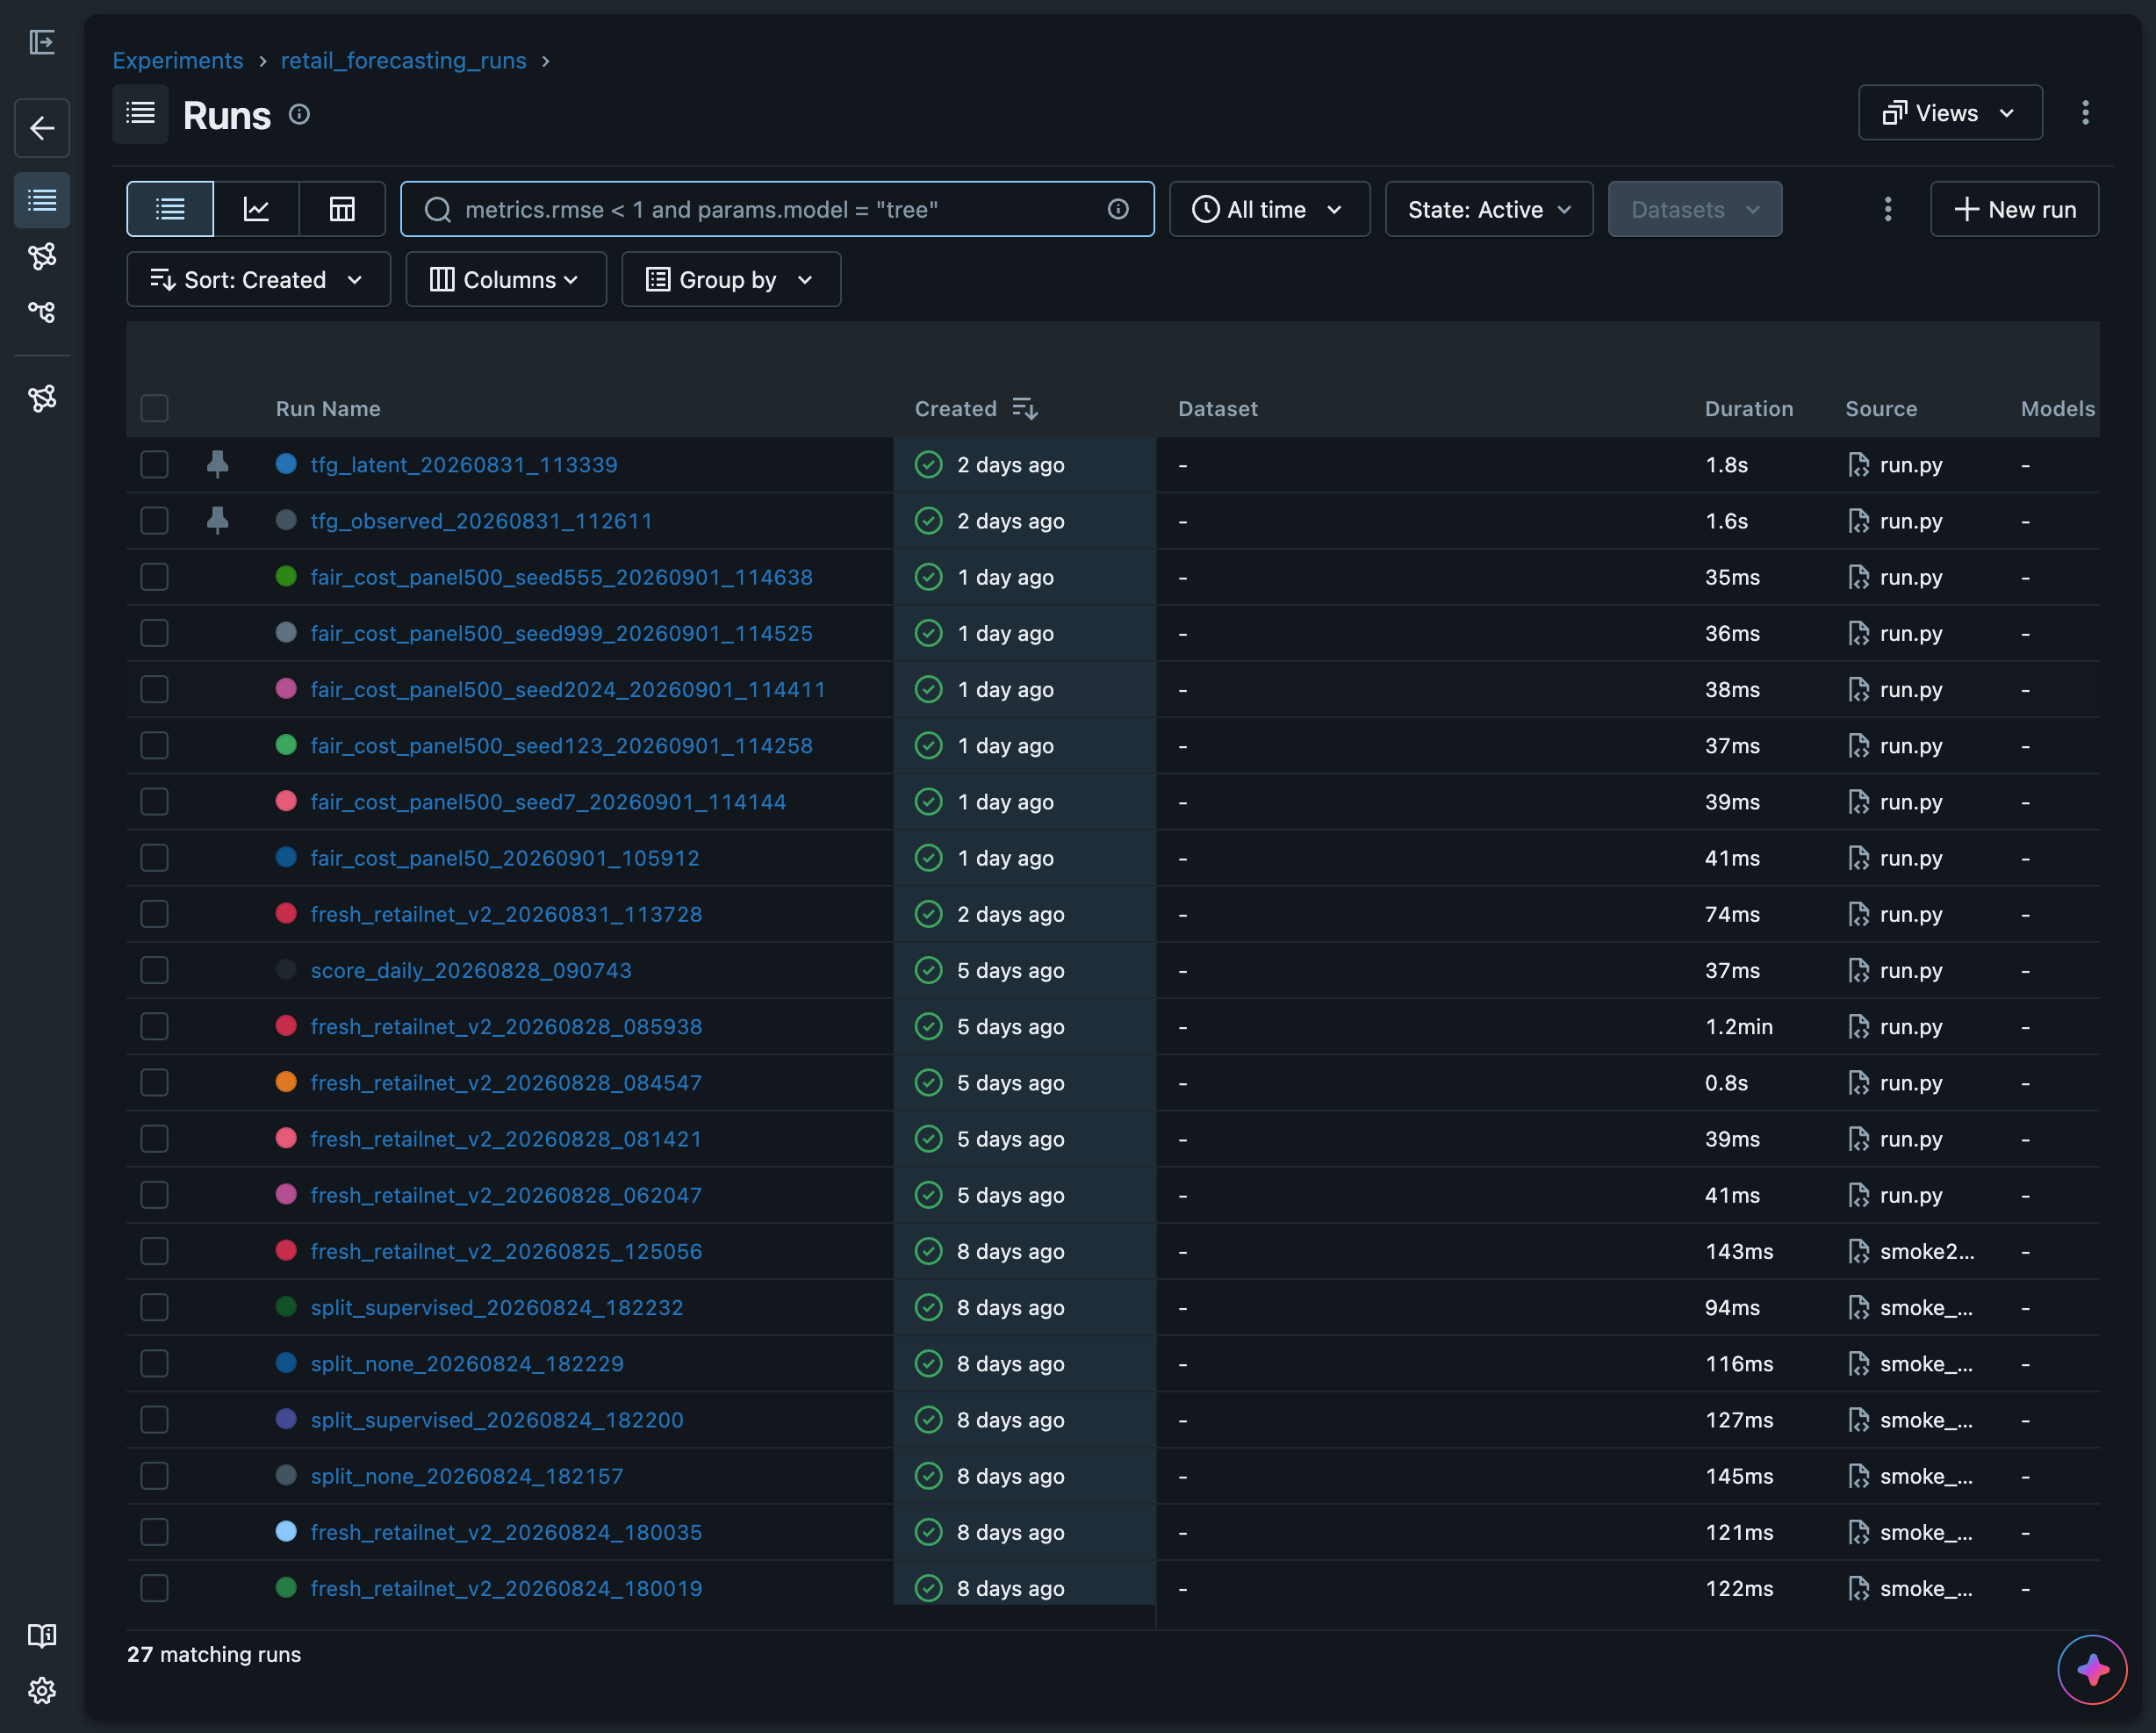
\includegraphics[width=\linewidth,height=0.72\textheight,keepaspectratio]{mlflow/mlflow_runs_table.png}
    \end{column}
    \begin{column}{0.46\textwidth}
      \begin{statbox}{Almacén de Corridas Versionado}{UPVNavy}
        \begin{itemize}\small
          \item Registro inmutable de \texttt{git\_commit}, \texttt{config\_hash} y semillas aleatorias.
          \item Persistencia de artefactos: predicciones, curvas de convergencia y métricas Newsvendor.
          \item Cualquier cifra de la memoria es 100\% reproducible por un tercero.
        \end{itemize}
      \end{statbox}
    \end{column}
  \end{columns}
\end{frame}

\end{document}
